\begin{frame}{Application: color segmentation}
K-means can be employed for image segmentation, simply by grouping pixels in the color space. You can also add coordinates to each pixel to obtain a smooth output.
\begin{figure}
\begin{tabular}{cc}
\small{Image} & \small{Segmentation}\\

\includegraphics[width=0.35\textwidth]{img/kmeans/emma.pdf}&
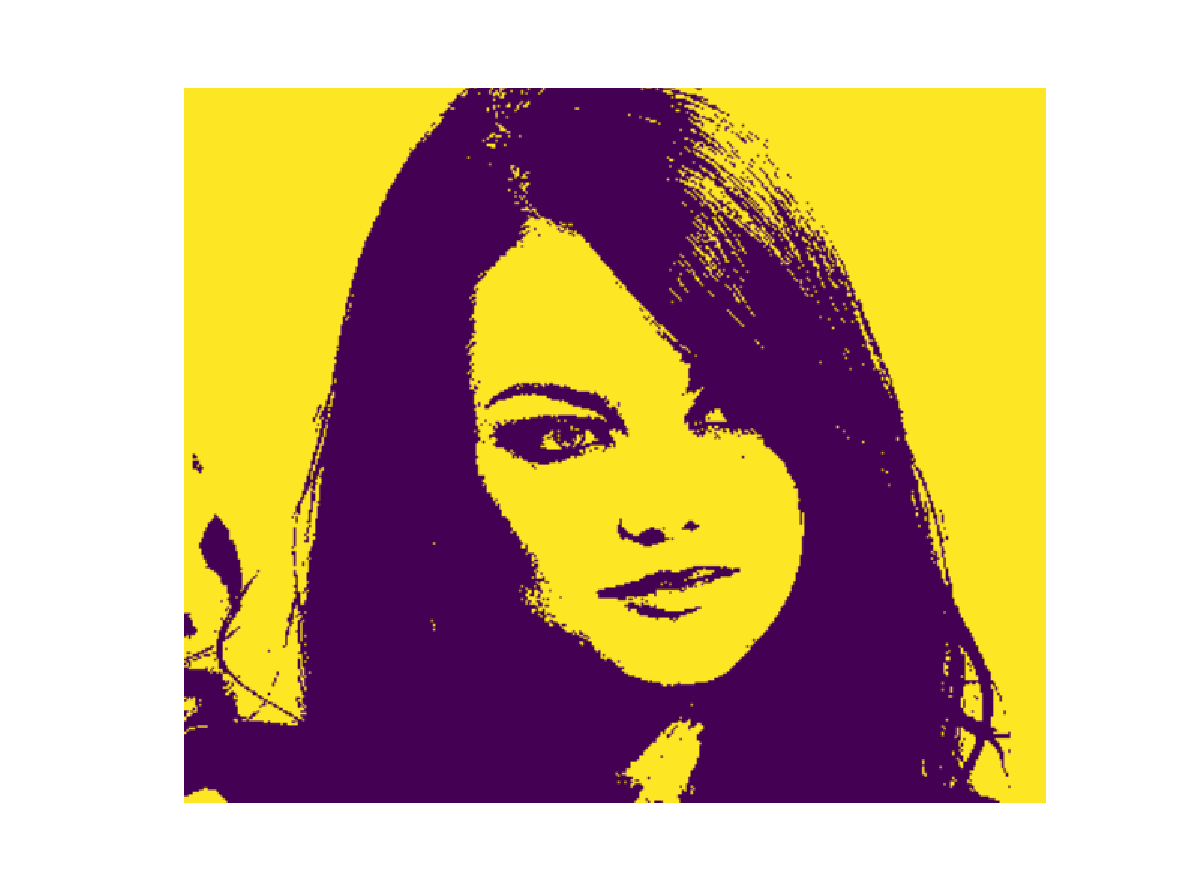
\includegraphics[width=0.35\textwidth]{img/kmeans/emma_segm.pdf}
\end{tabular}
\end{figure}
Try it!
\end{frame}